% !TeX root = RJwrapper.tex
\title{Assembling Pharmacometric Datasets in R - The \pkg{puzzle} Package} 
\author{by Mario Gonz\'alez-Sales*, Olivier Barri\`ere*, Pierre Olivier Tremblay, Guillaume Bonnefois, Julie Desrochers and Fahima Nekka }

\maketitle


\section*{Highlights}
\begin{itemize}
\item Pharmacometric analyses are integral components of the drug development process.
\item The time required to construct a pharmacometrics dataset can sometimes be higher than the effort required for the modeling \textit{per se}.
\item The puzzle package is the first open source tool developed to simplify and facilitate the time consuming and error prone task of assembling pharmacometrics datasets.
\item The datasets created using the puzzle package are compatible with the format requirements for the gold-standard non-linear mixed effects modeling software.
\item The puzzle package is available on CRAN.
\end{itemize}

\abstract{

\textbf{Background and objective:} Pharmacometric analyses are integral components of the drug development process. The core of each pharmacometric analysis is a dataset. The time required to construct a pharmacometrics dataset can sometimes be higher than the effort required for the modeling \textit{per se}. To simplify the process, the puzzle R package has been developed aimed at simplifying and facilitating the time consuming and error prone task of assembling pharmacometrics datasets.

\textbf{Methods:} Puzzle consist of a series of functions written in R. These functions create, from tabulated files, datasets that are compatible with the formatting requirements of the gold standard non-linear mixed effects modeling software.

\textbf{Results:} With only one function, \code{puzzle()}, complex pharmacometrics databases can easily be assembled. Users are able to select from different absorption processes such as zero- and first-order, or a combination of both. Furthermore, datasets containing data from one or more analytes, and/or one or more responses, and/or time dependent and/or independent covariates, and/or urine data can be simultaneously assembled. 

\textbf{Conclusions:} The puzzle package is a powerful and efficient tool that helps modelers, programmers and pharmacometricians through the challenging process of assembling pharmacometrics datasets.
}

\newpage


\section{Introduction}
The pharmacometrics workflow has routine steps: 1) assemble the dataset, 2) explore, 3) model the data, 4) evaluate, 5) validate the model, and 6) communicate the findings. The automation of these steps saves time and money, reduces the risk of errors, and increases reproducibility. Currently, a number of excellent tools are available to enhance steps 2-6~\citep{Jonsson1999, Lindbom2005, Keizer2011, Keizer2015, Mouksassi2016, Wang2016, Keizer2018, Xie2018, Mouksassi2019, Baron2019,RStudio}. However, to the best of our knowledge, there is no open source tool to support step 1). 
Considerable challenges exist when working in data management with an industrial setting that must comply with rules and regulations under the scrutiny and control of regulatory agencies, such as the U.S. Food and Drug Administration (FDA), Health Canada, the Japanese Pharmaceutical and Medical Device Agency (PMDA), or the European Medicines Agency (EMA). The task of dataset building should not be underrated, since the amount of time required to construct a pharmacometrics dataset can be sometimes higher than the effort required for the modeling \textit{per se}. In fact, it is often claimed that the process of cleaning and preparing the data could take up to 80\% of data analysis~\citep{Dasu2003}. In addition, data preparation does not amount to a single step, since it usually has to be repeated over the course of analysis as new data become available. 

Understanding the structure of pharmacometrics datasets is essential for an efficient data assembling. These datasets are two-dimensional arrangements of data in rows and columns. Each row represents a record or an event, while each column represents an item or a variable. Pharmacokinetic (PK) datasets are generally time-ordered arrangements of records representing the time course of plasma concentrations related to the dose of drug administered. Depending on the complexity of the system being modeled, pharmacodynamics (PD) datasets might or not include dose and/or time information. Furthermore, pharmacometrics datasets normally imply multiple doses, several routes of administration, different treated arms and/or sequences, time dependent and/or independent covariates, metabolite, and/or urine data, and/or information regarding one or multiple PD endpoints. These additional components tend to skyrocket the complexity of the data assembling as it makes the process hard to script up-front. This is especially true when working with data that are not in tidy shape~\citep{Wickham2014}. Due to this entanglement, complications are likely to happen throughout the process. In this regard, inconsistencies between exact dates, times of dose and blood sampling, different identifiers on the same requisition forms, imputation of missing and time-varying covariates, and missing timing of concomitant medications are common issues~\citep{Grasela2007}.

In this tutorial, we present the \pkg{puzzle} package to the pharmacometrics community, an open source tool for assembling pharmacometrics datasets in R. The \pkg{puzzle} package consists in a group of functions developed to simplify and facilitate the time consuming and error prone task of assembling pharmacometrics datasets. The datasets created are compatible with the formatting requirements of the NONMEM\textsuperscript{\textregistered}~software~\citep{Beal2009}. Moreover, as NONMEM\textsuperscript{\textregistered}~data structures are the gold standard for non-linear mixed effects modeling, the datasets created with the puzzle package are mostly compatible with other non-linear mixed effects softwares such as MONOLIX~\citep{Lixoft}, \pkg{saemix}~\citep{Comets2011},  and \pkg{nlmixr}~\citep{Fidler2019}.  The \pkg{puzzle} package is also available on CRAN and can be installed with the following R code: \code{install.packages("puzzle")}.

This tutorial proceeds as follows. First, we illustrate two common case studies of data assembling of pharmacometrics datasets using the \pkg{puzzle} package. Second, we dive into the arguments of the main function of the \pkg{puzzle} package, the \code{puzzle()} function. Third, we present the pre-formatting requirements of \code{puzzle()}, and finally, we conclude with a discussion regarding the limitations and inconveniences of this framework, and what are the other approaches or efforts that might be advantageous to pursue.

% or cite a reference such as \citet{R} in the text.
\section{Use of the \pkg{puzzle} function}

The  \code{puzzle()} function is flexible enough to build all types of pharmacometrics datasets in the appropriate format for the pharmacometrics analysis. The data presented in Figure~\ref{figure:fig1} will be used to show the readers the flexibility of the  \code{puzzle()} function and how powerful it is. In the first example, panels b, d, and e of Figure~\ref{figure:fig1} will be used to assemble a PK dataset containing parent and metabolite plasma concentrations, several covariates, and multiple administrations. The second example will imply panels a, c, d and f of Figure~\ref{figure:fig1}. The output dataset will be a PK/PD data set with time dependent covariates.

\begin{figure}[!ht]
  \centering
  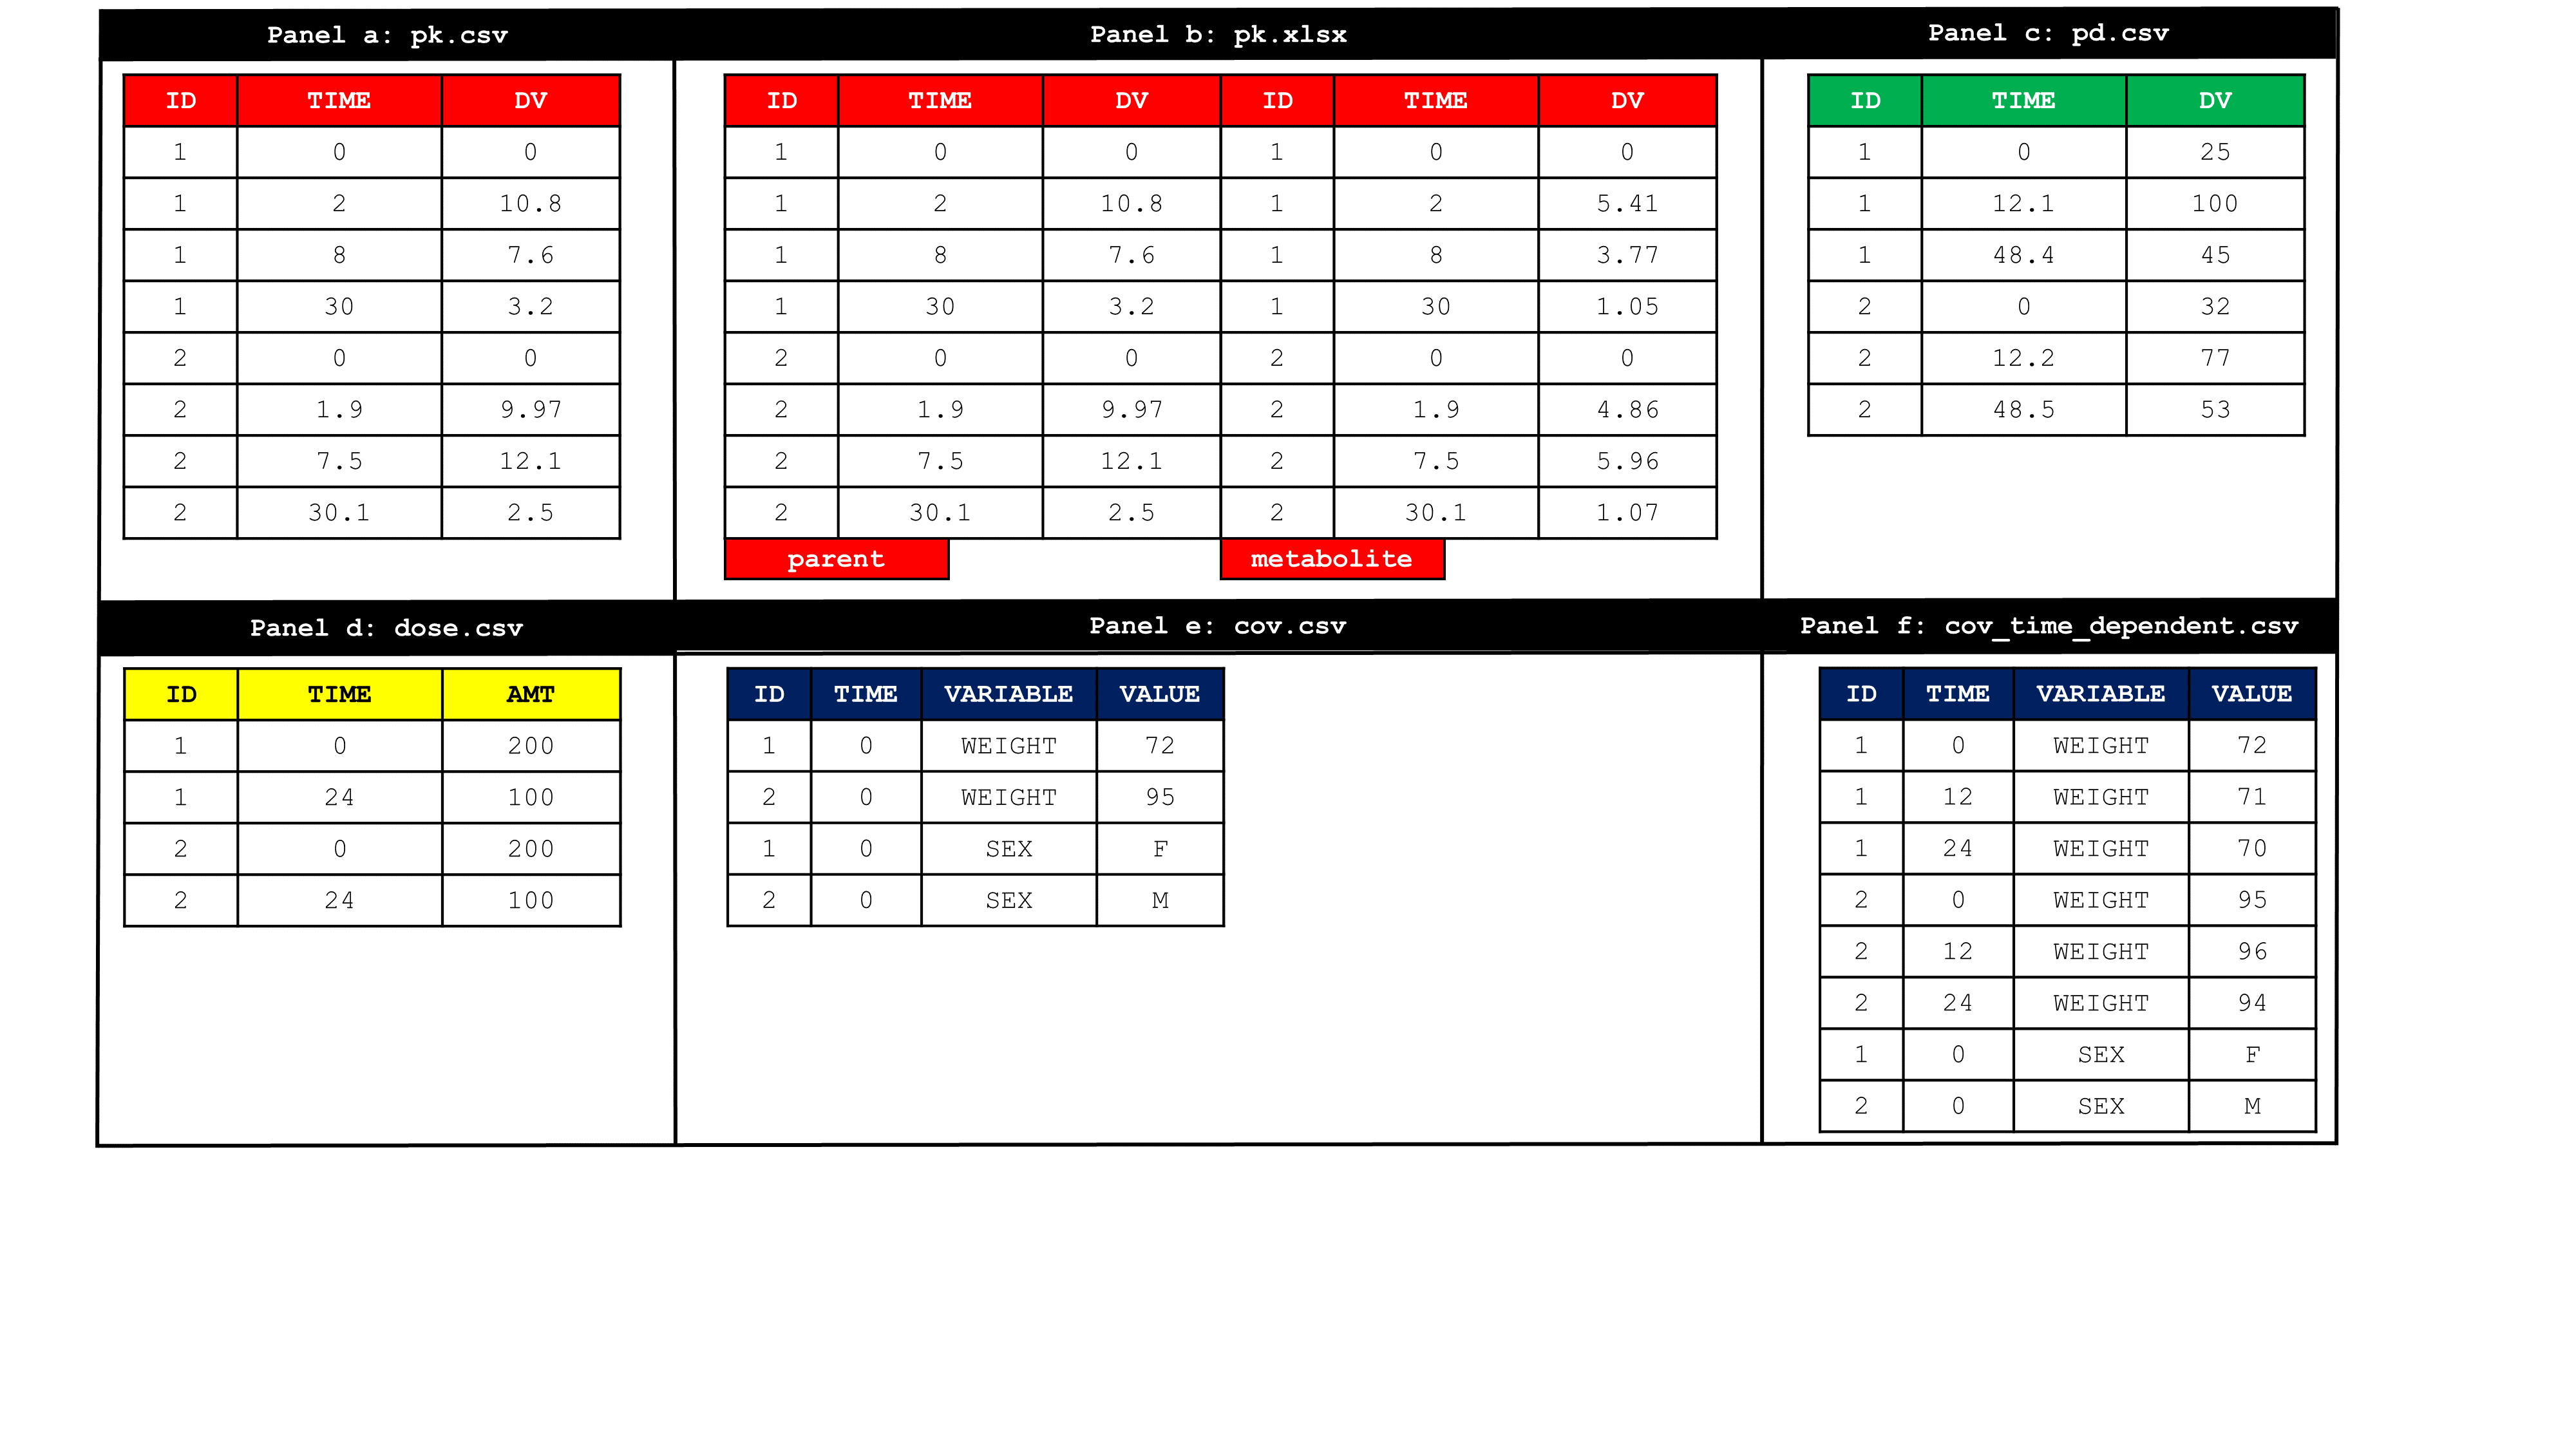
\includegraphics[trim=1.3cm 4cm 1.5cm 0cm,  clip=true, scale=0.70, angle =90]{Figure1}
   \caption{Structure of the four different files to input data into \code{puzzle()} function. \textit{Panels a and b illustrate the items required to input PK information from one and two analytes, respectively. Panel c and d depict the items to input PD and dosing information. Panel e and f presents the pre-formatting requirements to input covariate information assuming time in- and dependent covariates, respectively.}}
  \label{figure:fig1}
\end{figure}

\newpage

\textit{Example 1: PK data set}

The syntax to create the NM\_PK.csv depicted in Table~\ref{table:ex1} is as follows:
\begin{example}
library(puzzle)
directory = "C:/projects/puzzle/data"
puzzle(directory=file.path(directory),
       order=c(1,1),
       pk=list(name="pk.xlsx"), 
       dose=list(name="dose.csv"), 
       cov=list(name="cov.csv"), 
       nm=list(name="NM_PK.csv"),
       username="Mario Gonzales Sales")
       \end{example}
 
 \begin{table}[!ht]
\resizebox{\textwidth}{!}{ 
\begin{tabular}{|l|l|l|l|l|l|l|l|l|l|l|l|l|l|l|}
\toprule
\rowcolor{black}
\textcolor{white}{C} &	\textcolor{white}{ID}&	\textcolor{white}{TIME}&	\textcolor{white}{TAD}	&\textcolor{white}{DOSETIME}&	\textcolor{white}{PDOSETIME}&	\textcolor{white}{NUMDOSE}	&\textcolor{white}{AMT}&	\textcolor{white}{CMT}	&\textcolor{white}{EVID}	&\textcolor{white}{DV}&	\textcolor{white}{LDV}&	\textcolor{white}{MDV}	&\textcolor{white}{SEX}&	\textcolor{white}{WEIGHT} \\
\midrule
    &1	&0	&0	&0	&0	&1&	200	&1	&1	&.&	.	&1&	0&	72 \\
  \midrule
	&1	&0	&0	&0	&0	&1&	200	&2	&1	&.&	.	&1&	0&	72 \\
	\midrule
	&1	&0	&0	&0	&0	&1&	.	&3	&0	&0&	.	&0&	0&	72 \\ 
	\midrule
	&1	&0	&0	&0	&0	&1&	.	&4	&0	&0&	.	&0&	0&	72 \\
	\midrule
	&1	&2	&2	&0	&0	&1&	.	&3	&0	&10.8 &2.37954613 &	0&	0	&72 \\
	\midrule
	&1	&2	&2	&0	&0	&1&	.	&4	&0	&5.41&	1.68824909&	0&	0	&72 \\
	\midrule
	&1	&8	&8	&0	&0	&1&	.	&3	&0	&7.6&	2.02814825&	0&	0	&72 \\
\midrule
	&1	&8	&8	&0	&0	&1&	.	&4	&0	&3.77&	1.327075&	0&	0&	72 \\
	\midrule
	&1	&24	&0	&24	&0	&2&	100	&1	&1	&.&	.	&1	&0	&72 \\
	\midrule
	&1	&24	&0	&24	&24	&2	&100 &2	&1	&.&	.	&1	&0	&72 \\
\midrule
	&1	&30	&6	&24	&24	&2	&.	&3	&0	&3.2	&1.16315081	&0	&0&	72 \\
\midrule
	&1	&30	&6	&24	&24	&2	&.	&4	&0	&1.05&	0.04879016	&0	&0&	72 \\
	\midrule
	&2	&0	&0	&0	&0	&1	&200	&1&	1&	.&	.&	1&	1	&95 \\
\midrule
	&2	&0	&0	&0	&0	&1	&200	&2&	1&	.&	.&	1	&1	&95 \\
	\midrule
	&2	&0	&0	&0	&0	&1	&.&	3	&0	&0&	.&	0	&1	&95 \\
	\midrule
	&2	&0	&0	&0	&0	&1	&.	&4	&0	&0&	.&	0	&1	&95 \\
	\midrule
	&2	&1.9	&1.9&	0&	0&1	&.	&3&	0&	9.97&	2.29958058&	0	&1	&95 \\
	\midrule
	&2	&1.9	&1.9&	0&	0&	1	&.	&4&	0&	4.86&	1.58103844&	0	&1	&95 \\
	\midrule
	&2	&7.5	&7.5&	0&	0&	1	&.	&3&	0&	12.1&	2.49320545&	0	&1&	95 \\
	\midrule
	&2	&7.5	&7.5&	0&	0&	1	&.	&4&	0&	5.96&	1.78507048	&0	&1	&95 \\
	\midrule
	&2	&24 &	0	&24&	0&	2&	100	&1	&1&	.&	.	&1	&1	& 95 \\
	\midrule
	&2	&24	&  0	&24&	24&	2&	100	&2	&1&	.&	.	&1	&1	& 95 \\
	\midrule
	&2	&30.1	&6.1&	24&	24&	2	&.	&3&	0&	2.5	&0.91629073	&0	&1	&95 \\
	\midrule
	&2	&30.1	&6.1&	24&	24&	2	&.	&4&	0&	1.07&	0.06765865	&0	&1&	95 \\
	\bottomrule
\end{tabular}
}
 \caption{Returned output from the \code{puzzle()} function after running example 1 \label{table:ex1}} 
\end{table}
    
After running the \code{puzzle()} function the following message will be printed in the R console: 

\begin{example}
Automatic coercion to numeric for CMT
3=parent
4=metabolite
Automatic coercion to numeric for SEX
0=F
1=M
Assembling date and time: 2019-10-29 12:12:47
Time zone: Europe/Paris
Number of individuals: 2
Number of observations: 16
Dose levels: “100”, “200”
This data set was assembled by Mario Gonzalez Sales
\end{example}

It informs the user that parent and metabolite records are located in CMT 3 and 4, respectively. Moreover, it also indicates that the categorical variable SEX has been coerced into a numeric variable. Female (F) and male (M) categories have been assigned to the values of 0 and 1, respectively. The user should be aware that factors are coerced following alphabetical order. The date and time at which the dataset was assembled, the timezone where the assembling was performed, the number of individuals and observations in the dataset, the different dose levels administered, and if requested, the person who performed the data assembling will be automatically displayed. 

The  \code{puzzle()} function simultaneously assembles the PK (\textit{i.e.} parent and metabolite), the dose and the covariate information returning a NONMEM\textsuperscript{\textregistered}~ready dataset stored in a .csv file (\textit{i.e.} "NM\_PK.csv"). Because order has been set to \code{order = c(1,1)}, the dose has been split into two compartments (\textit{i.e.} CMT 1 and 2).  Furthermore, because there are two analytes, the observations have been assigned to an independent compartment (\textit{i.e.} CMT 3 and 4) for the parent and the metabolite, respectively. Additionally, the  \code{puzzle()} function automatically appends useful items to the output. Specifically, a placeholder to ignore records (C), time after dose (TAD), dosing time (DOSETIME), prior dosing time (PDOSETIME), the compartment item (CMT), the event identification (EVID), the log of the DV (LDV) and the missing dependent variable item (MDV).  

\textit{Example 2: PK/PD data set}

The syntax to create the NM\_PKPD.csv depicted in Table~\ref{table:ex2} is as follows:
\begin{example}
puzzle(directory=file.path(directory),
       order=0,
       pk=list(name="pk.csv"), 
       pd=list(name="pd.csv"), 
       dose=list(name="dose.csv"), 
       cov=list(name="cov_time_dependent.csv"),
       coercion=list(name="coercion.txt"),
       nm=list(name="NM_PKPD.csv"))
       \end{example}

 
\begin{table}[!ht]
\resizebox{\textwidth}{!}{ 
\begin{tabular}{|l|l|l|l|l|l|l|l|l|l|l|l|l|l|l|l|}
\toprule
\rowcolor{black}
\textcolor{white}{C} &	\textcolor{white}{ID}&	\textcolor{white}{TIME}&	\textcolor{white}{TAD}	&\textcolor{white}{DOSETIME}&	\textcolor{white}{PDOSETIME}&	\textcolor{white}{NUMDOSE}	&\textcolor{white}{AMT}&	\textcolor{white}{TYPE}	&	\textcolor{white}{CMT}	&\textcolor{white}{EVID}	&\textcolor{white}{DV}&	\textcolor{white}{LDV}&	\textcolor{white}{MDV}	&\textcolor{white}{SEX}&	\textcolor{white}{WEIGHT} \\
\midrule
  	&1	&0	&0	&0	&0	&1	&200	&0	&1	&1	&.&	.&	1&	0&	72\\
  \midrule
	&1	&0	&0	&0	&0	&1	&.	&1	&1	&0	&0	&.	&0	&0	&72\\
\midrule
	&1	&0	&0	&0	&0	&1	&.	&2	&2	&0	&25	&3.21887582	&0	&0	&72\\
	\midrule
	&1	&2	&2	&0	&0	&1	&.	&1	&1	&0	&10.8	&2.37954613	&0	&0	&72\\
	\midrule
	&1	&8	&8	&0	&0	&1	&.	&1	&1	&0	&7.6	&2.02814825	&0	&0	&72\\
	\midrule
	&1	&12.1	&12.1	&0	&0	&1	&.	&2	&2	&0	&100	&4.60517019	&0	&0	&71\\
	\midrule
	&1	&24&	0	&24&	0	&2	&100	&0	&1	&1	&.	&.	&1	&0	&70\\
	\midrule
	&1	&30&	6	&24	&24&	2	&.	&1	&1	&0	&3.2	&1.16315081	&0	&0	&70\\
	\midrule
	&1	&48.4	&24.4	&24	&24&	2	&.	&2	&2	&0	&45	&3.80666249	&0	&0	&70\\
\midrule
	&2	&0	&0	&0	&0	&1	&200	&0	&1	&1	&.	&.	&1	&1	&95\\
	\midrule
	&2	&0	&0	&0	&0	&1	&.	&1	&1	&0	&0	&.	&0	&1	&95\\
	\midrule
	&2	&0	&0	&0	&0	&1	&.	&2	&2	&0	&32	&3.4657359	&0	&1	&95\\
	\midrule
	&2	&1.9	&1.9	&0	&0	&1	&.	&1	&1	&0	&9.97	&2.29958058	&0	&1	&95\\
\midrule
	&2	&7.5	&7.5	&0	&0	&1	&.	&1	&1	&0	&12.1	&2.49320545	&0	&1	&95\\
	\midrule
	&2	&12.2	&12.2	&0	&0	&1	&.	&2	&2	&0&	77	&4.34380542	&0	&1&	96\\
	\midrule
	&2	&24&	0	&24&	0	&2	&100&	0	&1	&1	&.	&.	&1	&1&	94\\
	\midrule
	&2	&30.1&	6.1&	24&	24&	2	&.	&1	&1	&0	&2.5&	0.91629073	&0	&1	&94\\
	\midrule
	&2	&48.5&	24.5&	24	&24&	2	&.	&2	&2	&0	&53	&3.97029191&	0	&1	&94\\
	\bottomrule
\end{tabular}
}
\caption{Returned output from the \code{puzzle()} function after running example 2 \label{table:ex2}} 
 \end{table}
   
In this case, the variable type of observation (\textit{i.e.} TYPE) has been appended to the "NM\_PKPD.csv" file. Because a bolus administration has been specified with the argument \samp{order} (\textit{i.e.} \code{order = 0}), TYPE has a value of 0 for dosing events, and a value of 1 and 2 for PK and PD records, respectively.  Moreover, the file "coercion.txt" has been generated. The content is printed below:

\begin{example}
CMT: 1=pk, 2=pd
SEX: 0=F, 1=M
\end{example}

\section{The argument of the \pkg{puzzle} function}

The \code{puzzle()} function builds pharmacometrics ready datasets from a group of tabulated files. For convenience, it always returns a ".csv" file or an R object of class "data.frame" as output. The path to the location of the files to be assembled can be set with the \samp{directory} argument. Depending on the pharmacometric analysis to be performed, the tabulated files may contain PK, dose, covariates and/or PD information. 

The PK data may include drug concentration (\textit{i.e.} parent and/or metabolite/s) and/or urine information. The \samp{pk} argument is used to input this type of data into the \code{puzzle()} function. The general form is as follows: 
\begin{example}
pk = list(name = NULL, data = NULL) 
\end{example}

If the PK data is stored in a ".csv" or an ".xlsx" file, the name of the file should be provided with name:
\begin{example}
pk = list(name = "pk.csv", data = NULL) 
\end{example}

Alternatively, if the data is within the R environment, the name of the R object may be defined with the parameter data: 
\begin{example}
pk = list(name = NULL, data = nm$pk) 
\end{example}

where \samp{nm} is a list containing the PK information \samp{pk}. Excel files are useful to simultaneously store PK information from two or more analytes. The  \code{puzzle()} function is smart enough to assemble all the PK information at once. To this end, each analyte data has to be contained in its own spreadsheet. Moreover, each sheet has to have the same items, and the items have to be in the same order. 


The PD information may comprise the time course of the clinical endpoint of interest, time to event data, and/or a response outcome. This type of information is handled with the \samp{pd} argument. Its behavior is similar to \samp{pk}, and thus, it accepts the same type of tabulated files and it requires a similar syntax. For example, in case of multiple endpoints stored in an ".xlsx" file, the user should define: 
\begin{example}
pd = list(name = "pd.xlsx", data = NULL)  
\end{example} 
or simply
\begin{example}
pd = list(name = "pd.xlsx")
\end{example}

Consistently, covariate and dose information are inputted to the \code{puzzle()} function with the arguments \samp{cov} and \samp{dose}, respectively. The reader should note that ".xlsx" files are not required, and the data should be contained within a ".csv" file or an R object. Finally, \samp{extratimes} is another argument following this logic. This argument can be used to add a common pattern of additional times for each individual within the dataset. The user may be interested in this feature for prediction purposes. For example, if the data are very sparse (\textit{i.e.} 2 observations per individual from time 1 to 4 hours post drug administration), it is possible to define a vector of times from time 0 to 4 hours post dose in order to obtain a smooth prediction (\textit{e.g.} \code{extratimes = list(name = "extratimes.csv", data = NULL)} ). Of note, EVID = 2 will be assigned to these extra times.

The \samp{cov} and \samp{dose} arguments may be used in combination with a number of additional arguments: \samp{optionalcolumns}, which defines the optional columns to be appended in to the output. For instance, if more than one treatment is administered, the file storing the dose information may contain the variable treatment (\textit{i.e.} "TRT"). If the user wants to include this variable in the pharmacometrics dataset, the following syntax is warranted:  \code{optionalcolumns = "TRT"}. If more than one variable are to be appended, the syntax should be:  \code{optionalcolumns = c("variable 1", "variable 2")}.
Furthermore, the argument \samp{fillcolumns} fills the columns appended with the argument \samp{optionalcolumns} using the last observation carried forward method. If the argument is defined as \code{fillcolumns = "TRT"}, the variable TRT will be added without missing values. Otherwise, the value of TRT only will be available for dosing records, and non-dosing records will be outputted as ".", the default for missing values. 

The \code{puzzle()} function is able to coerce numeric variables from character variables. If a character variable is introduced with the \samp{cov} argument, this variable will be automatically coerced into a numeric variable. For example, let’s assume we have a character variable accounting for renal impairment with the following possible values: "mild", "moderate" and "severe". The \code{puzzle()} function will convert the variable from character to factor. Each string will be a different level. Then, the factor variable will be coerced into numeric. If there is no numeric order within the factor, the levels will be alphabetically assigned. The argument \samp{initialindex} defines the initial value of the coerced numeric variable. The default value is \code{initialindex = 0}. Therefore, under the default settings, the "mild", "moderate" and "severe" levels will have numeric values of 0, 1 and 2, respectively. Moreover, a string for missing values can be defined with the argument \samp{na.strings}. Thus, if a variable has a missing value, this can be labeled as not available as follows: \code{na.strings = "N/A"}.  For convenience, a ".txt" file may be created with the argument \samp{coercion}. This argument creates a record of the categories of each coerced variable. If the user defines \code{coercion = list(name = "my\_coercion\_records.txt")}, a file with the name "my\_coercion\_records.txt" will be generated in the working directory after running the \code{puzzle()} function. The user can also control the variables to be included in the records with the argument \samp{nocoercioncolumns}. 

When performing population PK analysis in NONMEM\textsuperscript{\textregistered}, the structure of the data set depends on the route of administration. This implies that the data structure is different for bolus, infusion and oral administrations~\citep{Owen2014}.  The argument \samp{order} is used to handle this situation. It can take four different values: \code{order = 0} indicates a zero-order absorption process. It may be used for bolus or infusion administrations. For the later, the RATE has to be given in the dosing file; \code{order = 1} serves to generate datasets to model first-order absorption processes (\textit{e.g.} oral administration); \code{order = c(1,1)} may be used to model the absorption of drugs with complex formulations. An example may be a drug formulated as immediate and extended release. In this situation, two different absorption rates may be warranted, and \code{c(1,1)} means that the dataset is built assuming two first-order absorption processes. Finally, \code{order = c(0,1)} allows the user to define a zero- and first-order absorption processes. By default, the \code{puzzle()} function assumes this process occurs in parallel, meaning that one fraction of the drug is absorbed thorough a zero-order process and the remaining amount of the drug is absorbed following a first-order process. However, it may also follow a sequential process where the drug is delivered thorough a zero-order process to the depot compartment, and then, absorbed into the bloodstream following a first-absorption process. The argument \samp{parallel} can be set to false (\textit{i.e.} \code{parallel = FALSE)} to control these absorption patterns. The user must be aware that if order is not set to \code{order = c(0,1)} and \code{parallel = FALSE}, \code{puzzle()} will return the following error message: 


\textcolor{red}{
Error in puzzle(directory = file.path(getwd()), order = c(1, 1), parallel = F,: 
Would you like to use a sequential zero + first order absorption model? 
Please set order=c(0,1). Otherwise, please set parallel = T
}

A characteristic of the NONMEM\textsuperscript{\textregistered}~datasets is that characters are not allowed, and all the items, except DAT, must be numeric. Hence, the command IGNORE in the \$INPUT block within a NONMEM\textsuperscript{\textregistered}~control stream is commonly used to ignore the label of the data items. The \code{puzzle()} function has the argument \samp{ignore} to create a new item for this purpose. For example, if the user sets ignore = "C", the first column of the returned ".csv" file will contain an item called C. The argument \samp{missingvalues} allows the user to specify a label for the missing values. The default value is \code{missingvalues = "."}.

The user can control how the records are arranged with the argument \samp{arrange}. By default, records are arranged as follows: \code{arrange="ID,TIME,CMT,desc(EVID)"}. Moreover, complex date formatting is also supported. The argument \samp{datetimeformat} defines the format for dates and times. By default, the format is \code{datetimeformat = "\%Y-\%m-\%d \%H:\%M:\%S"}. In addition to that, time units may be specified with the argument  \samp{timeunits}. For example, \code{timeunits = "hours"}. It should be highlighted that the timezone will affect how times are computed from dates. Thus, depending on your location, times may be slightly different because the default value is \code{timezone = Sys.timezone()}. The user can also identify the person assembling the dataset with the argument \code{username}. The last argument of the \code{puzzle()} function is \samp{nm}. It is used to name the output from the function, in other words, the returned ".csv" file. The syntax of the arguments of the  \code{puzzle()} function is presented in Table~\ref{table:syntax}.

\begin{table}[!ht]
\begin{tabular}{c|l}
\toprule
Argument	 & Example of syntax\\
\midrule
directory	 & \code{directory = file.path(getwd()) }\\
pk 	 & \code{pk = list(name="pk.csv")}\\
pd	 & \code{pd = list(name="pd.csv")}\\
cov	 & \code{cov = list(name="cov.csv")}\\
dose  & 	\code{dose = list(name="dose.csv")}\\
extratimes 	 & \code{extratimes = list(name="extratimes.csv")}\\
optionalcolumns	 & \code{optionalcolumns = "TRT"}\\
fillcolumns	 & \code{fillcolumns = "TRT"}\\
initialindex & 	\code{initialindex = 0}\\
na.strings	 & \code{na.strings = "N/A"}\\
coercion & 	\code{coercion = list(name = "coercion.txt")}\\
nocoercioncolumns	& \code{nocoercioncolumns = NULL}\\
order	& \code{order = c(0,1)}\\
parallel	& \code{parallel = FALSE}\\
ignore& 	\code{ignore = "C"}\\
missingvalues	& \code{missingvalues = "."}\\
arrange	&\code{arrange = "ID,TIME,CMT,desc(EVID)"}\\
datetimeformat& 	\code{datetimeformat="\%Y-\%m-\%d \%H:\%M:\%S" }\\
timeunits	& \code{timeunits="hours" }\\
timezone	& \code{timezone=Sys.timezone()} \\
username & \code{Username="User"} \\
nm &  	\code{nm=list(name="NONMEM.csv")}\\
\bottomrule
\end{tabular}
\caption{Syntax of the arguments of the \code{puzzle()} function  \label{table:syntax}}
\end{table}

\section{Pre-formatting requirements}

At the beginning of a new project, the modeler or the programmer usually faces a series of large and structurally diverse datasets where the required information for the analysis is stored. It is a common practice that data are collected using automatic informatics methods. Unfortunately, the systems may storage the information in multiple and non-tidy pre-defined files. This situation is not ideal to assemble the pharmacometrics datasets because the programmer has to spend valuable time puzzling out and assembling all the heterogeneous information. The \code{puzzle()} function generates NONMEM\textsuperscript{\textregistered}~formatted datasets from standard tabulated files. Consequently, before calling the \code{puzzle()} function, it may be necessary to perform some data manipulation~\citep{Wickham2016,Chen2017}.  The degree of data manipulation will depend on the structure of the stored information. Given the high combination of possible data structures, detailing how the data should be manipulated is out of the scope of this manuscript. The reader is referred to the documentation of the \pkg{tidyverse} package for more information regarding how to efficiently perform this step~\citep{Wickham2017}.   

Pharmacometrics datasets usually contain PK, PD, dose and/or covariate information. The \code{puzzle()} function requires each type of information to be inputted from a separate tabulated file. Each file has to contain pre-defined variables with specific labels.

\subsection{Pre-formatting requirements for the tabulated file containing the PK information}

This file has to have at least three columns: i) a column used for subject identification "ID"; ii) a column containing the sampling times at which the PK samples were collected "TIME" or "DATETIME"; and iii) the observed value of the dependent variable "DV". The tabulated file can be an R object of class list, or a ".csv" file in case of assembling data from one analyte (Figure~\ref{figure:fig1}: panel a). If information from more than one analyte is to be assembled (Figure~\ref{figure:fig1}: panel b), the data should be stored in an ".xlsx", or in an R object of class list. For example, if parent and metabolite information are available, the \code{puzzle()} function requires an ".xlsx" file with one sheet containing the PK information of the parent drug, and another sheet storing the PK information of the metabolite. There is no limit in the number of sheets that the \code{puzzle()} function can handle. However, it is mandatory that each sheet includes the three pre-defined columns mentioned above. 

\subsection{Pre-formatting requirements for the tabulated file containing the PD information}

The \code{puzzle()} function has the same requirements for the PD than for the PK information. Therefore, the same three items (\textit{i.e.} ID, TIME or DATETIME, and DV) are mandatory and depending on the number of PD endpoints available, the data can be stored in an R object of class list, a ".csv" or an ".xlsx" file (Figure~\ref{figure:fig1}: panel c). 

\subsection{Pre-formatting requirements for the tabulated file containing the dosing records}
At least three columns are required: i) a column used as subject identification "ID": ii) a column containing the times at which the doses were administered "TIME" or "DATETIME"; and iii) the given dose "AMT" (Figure~\ref{figure:fig1}: panel d). In addition to that, and depending on the study design, other columns may be present as well. Later on, these columns may be passed to the returned ".csv" file using the \samp{optionalcolumns} argument.


\subsection{Pre-formatting requirements for the tabulated file containing the covariate information}

If this file is used, it has to include the following three items: i) a column with subject identification "ID"; ii) the name of the variable "VAR", and iii) the value of the variable "VALUE" (Figure~\ref{figure:fig1}: panel e). Of note, the \code{puzzle()} function is able to handle time independent (\textit{e.g.} sex) or time dependent covariates (Figure~\ref{figure:fig1}: panel f). In the specific case of time dependent covariates, a fourth item is mandatory: iv) a column containing the times at which the covariates were collected "TIME" or "DATETIME". This is required so that the  \code{puzzle()} function can know the times at which the value of the covariate changes within a subject.


\section{Discussion}
The \pkg{puzzle} package has been designed to be used as simple as possible. In fact, with a few lines of R code, modelers, programmers and overall pharmacometricians have now an open source tool to assemble complex pharmacometrics datasets. In order to facilitate its use and to decrease the slope of the learning curve, users are only required to learn the behavior and syntax of one function, \code{puzzle()}. Nevertheless, the \pkg{puzzle} package involves additional functions intentionally working "under the hood" to enhance the user experience. These functions are borrowed from several R libraries including: utils, lubridate, stats, readxl, reshape2, sqldf, plyr, and dplyr. The \pkg{puzzle} package started to be coded more than six years ago. At the time, reshape2, plyr, readxl and sqldf were useful tools from a data assembling perspective. However, if the \pkg{puzzle} package was started to be coded from scratch nowadays, the authors would probably use the \pkg{tidyverse} package as reference. 

At first, the main inconvenience of \code{puzzle()} may be the requirement of specific pre-defined formatting for its inputs. Nevertheless, it is indeed this feature that drastically increases the flexibility and productivity of \code{puzzle()}, allowing the assembling of all types of pharmacometrics datasets. The examples provided herein only scratches the surface of what the package is able to do. The reader is referred to the supplementary material for additional examples on how assembling pharmacometrics datasets using the \pkg{puzzle} package. 

The data assembling workflow starts with data collection. The second step is data storage. Unfortunately, most of the heterogeneity and difficulty during the data assembling arises in this step. Effectively, each company or hospital may use its own recipe to store the data. Even more complexity is usually added to the process if, within a company or hospital, different scientists or nurses are involved in the data collection and/or storage. This is due to inter-individual (\textit{i.e.} "two persons may label the same item differently") and/or inter-occasion (\textit{i.e.} "the same person may label the same item differently") variability. This fact makes the principle of reproducibility from a data preparation point of view quite challenging. 

The use of Study Data Tabulation Model (SDTM) has provided a standard for organizing and formatting data to streamline processes in collection, management, analysis and reporting, and it is one of the required standards for data submission to FDA and PMDA. The submission data standards team of Clinical Data Interchange Standards Consortium (CDISC) defines SDTM~\citep{DISC}.  On July 21, 2004, SDTM was selected as the standard specification for submitting tabulation data to the FDA for clinical trials and on July 5, 2011 for nonclinical studies. 

Unfortunately, inconsistencies in the data are not uncommon even if strict rules are supposed to be followed. Because of the heterogeneity of the data being assembled, the main limitation of the \pkg{puzzle} package is the requirement of pre-data manipulation. Specifically, the inconsistencies from SDTM have to be cleared before its use. Thus, at this stage of the development, the \pkg{puzzle} package is not fully compatible with SDTM datasets. Nevertheless, it is planned to implement this feature in the next version of the package. Alternatively, maybe, it is time within the pharmacometrics community to go one step further and develop new tools and methods allowing the establishment of strategies and/or protocols where data are more homogeneously stored. If this objective is accomplished and the degree of pre-data manipulation is reduced or even completely eliminated, the often-painful process of data assembling may become a breeze. 

\section{Conclusion}
The \pkg{puzzle} package is a very flexible, powerful and efficient tool that helps modelers, programmers and/or pharmacometricians through the complex model building process. Specifically, it is the first open source tool supporting pharmacometricians during the difficult, error prone, and time consuming process of data assembling. Therefore, the \pkg{puzzle} package fills an unmet condition within the pharmacometrics workflow as it offers an opportunity for a unification of the code for data assembly improving reproducibility and traceability. Thus, we do believe that the \pkg{puzzle} package will be of high interest for the pharmacometrics community. It is the authors hope that this manuscript serves as detonating to set the foundations for a more efficient and pleasant data assembling in our field.

\bibliography{gonzalez-sales-mario}

\address{Mario Gonz\'alez Sales*\\
 Modeling Great Solutions\\
 Crta. Engolasters s/n, Escaldes-Engordany, AD700\\
 Andorra\\
  \email{mario@modelinggreatsolutions.com}}

\address{Olivier Barri\`ere*\\
  Certera\\
2000 Peel Street, Suite 570, Montr\'eal, H3A 2W5 \\
  Canada\\
  \email{olivier.barriere@certara.com}}
  
  *Both authors share the first authorship. 

\address{Pierre Olivier Tremblay\\
 Syneos Health\\
  2500 Rue Einstein, Qu\'ebec, G1P 0A2\\
  Canada\\
  \email{pierreolivier.tremblay@syneoshealth.com}}
  
\address{Guillaume Bonnefois\\
 Syneos Health\\
 5160, boulevard D\'ecarie, Montr\'eal, H3X 2H9\\
   Canada\\
  \email{guillaume.bonnefois@syneoshealth.com}}
  
\address{Julie Desrochers\\
  Syneos Health, Qu\'ebec, Canada\\
  2500, Rue Einstein, Qu\'ebec, G1P 0A2\\
   Canada\\
  \email{julie.desrochers@syneoshealth.com}}
  
  
\address{Fahima Nekka \\
  Universit\'e de Montr\'eal - Facult\'e de Pharmacie \\
  2940, Chemin de Polytechnique, Montr\'eal, H3T 1J4\\
   Canada\\
  \email{fahima.nekka@umontreal.ca}}